\begin{frame}
    \frametitle{Reactor Numbers}
    \begin{table}
        \centering 
        \caption{Maximum number of reactors deployed at one time in 
        Scenarios 2-7.}
        \label{tab:reactors_nogrowth}
        \begin{tabular}{c c c c c}
            \hline
            Scenario & \glspl{MMR} [\#] & Xe-100s [\#] & VOYGRs [\#] 
            & Total [\#]\\\hline
            2 & 17,892 & - & - & 17,892\\
            3 & - & 1,119 & - & 1,119\\
            4 & 628 & 1,079 & - & 1,707\\
            5 & 628 & - & 1,122 & 1,749\\
            6 & - & 1,045 & 77 & 1,122\\
            7 & 472 & 1,082 & 7 & 1,561\\
            \hline
        \end{tabular}
    \end{table}
\end{frame}

\begin{frame}
    \frametitle{Enriched uranium masses}
    \begin{table}
        \centering 
        \caption{Metrics for enriched uranium sent to advanced 
        reactors between 2025-2090 in Scenarios 2-7.}
        \label{tab:nogrowth_uranium}
        \begin{tabular}{l p{2cm} p{2cm} p{2cm} p{2cm}}
            \hline
            Scenario & Average (MT/month) & \gls{HALEU} Average 
            (MT/month) & Maximum (MT)& Cumulative (MT)\\\hline
            2 & 88.90 & 88.90 & 1,007 & 69,251\\
            3 & 31.64 & 31.64 & 86.79 & 24,646\\
            4 & 33.62 & 33.62 & 101.5 & 26,193\\
            5 & 152.3 & 3.070 & 581.1 & 118,608\\
            6 & 39.92 & 29.51 & 103.3 & 31,095\\
            7 & 33.85 & 32.97 & 103.0 & 26,370\\
            \hline
        \end{tabular}
    \end{table}
\end{frame}

\begin{frame}
    \frametitle{Feed uranium masses}
    \begin{table}
        \centering 
        \caption{Metrics for feed uranium required by advanced reactors 
        between 2025-2090 in Scenarios 2-7.}
        \label{tab:nogrowth_feed}
        \begin{tabular}{l p{2cm} p{2cm} p{2cm} p{2cm}}
            \hline
            Scenario & Average (MT/month) & \gls{HALEU} Average 
            (MT/month) & Maximum (MT) & Cumulative (MT)\\\hline
            2 & 3,401 & 3,401 & 38,517 & 2,649,436\\
            3 & 947.3 & 947.3 & 2,598 & 737,950\\
            4 & 1,032 & 1,032 & 3,171 & 804,647\\
            5 & 1,253 & 117.5 & 4,668 & 976,207\\
            6 & 962.9 & 883.7 & 2,681 & 750,072\\
            7 & 1,013 & 1,007 & 3,228 & 789,745\\
            \hline
        \end{tabular}
    \end{table}
\end{frame}

\begin{frame}
    \frametitle{SWU capacity}
    \begin{table}
        \centering 
        \caption{Metrics for \gls{SWU} capacity to enrich uranium for 
        advanced reactors between 2025-2090 in Scenarios 2-7.}
        \label{tab:nogrowth_swu}
        \begin{tabular}{l p{2cm} p{2cm} p{2cm}}
            \hline
            Scenario & Average  (MT-SWU/month) & Average
            for \gls{HALEU} (MT-SWU/month) & Maximum (MT-SWU)\\\hline
            2 & 4,010 & 4,010 & 45,424 \\
            3 & 1,090 & 1,090 & 2,991\\
            4 & 1,192 & 1,192 & 3,668\\
            5 & 1,145 & 138.5 & 4,228 \\
            6 & 1,087 & 1,017 & 3,050\\
            7 & 1,167 & 1,161 & 3,735\\
            \hline
        \end{tabular}
    \end{table}
\end{frame}

\begin{frame}
    \frametitle{SNF discharged}
    \begin{table}
        \centering 
        \caption{Metrics for waste discharged from advanced reactors 
        between 2025-2090 in Scenarios 2-7.}
        \label{tab:nogrowth_waste}
        \begin{tabular}{l p{2cm} p{2cm} p{2cm} p{2cm}}
            \hline
            Scenario & Average (MT/month) & Average of \gls{HALEU} 
            (MT/month) & Maximum (MT) & Cumulative (MT)\\\hline
            2 & 66.15 & 66.15 & 1,142 & 51,531\\
            3 & 32.93 & 32.93 & 55.29 & 25,654\\
            4 & 34.07 & 34.07 & 77.55 & 26,543\\
            5 & 144.9 & 2.294 & 377.0 & 112,913\\
            6 & 40.68 & 30.72 & 75.12 & 31,691\\
            7 & 34.46 & 33.62 & 83.14 & 26,848\\
            \hline
        \end{tabular}
    \end{table}

\end{frame}

\begin{frame}
    \frametitle{Effect of capacity factors}
    \begin{figure}
        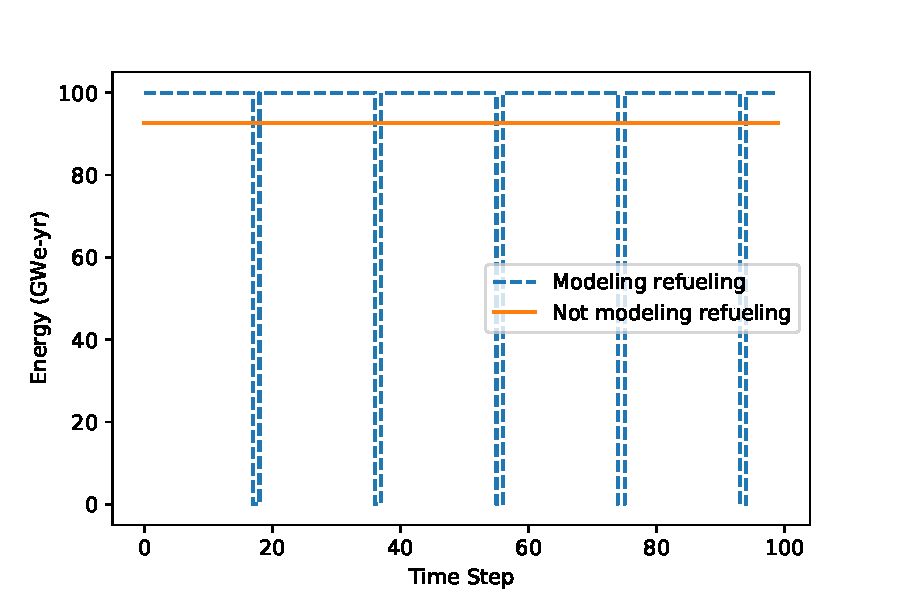
\includegraphics[scale=0.5]{CF_demo.pdf}
        \caption{Demonstration of the effect of not explicitly modeling 
        refueling outages on energy generated.}
        \label{fig:CF}
\end{figure}
\end{frame}